\documentclass{article}
\usepackage[T1]{fontenc}
\usepackage{lmodern}
\usepackage{graphicx}
\usepackage{amsmath,amssymb}
\usepackage[a4paper,margin=2cm]{geometry}
\usepackage[absolute,overlay]{textpos}
\setlength{\TPHorizModule}{1mm}
\setlength{\TPVertModule}{1mm}
\usepackage[indonesian]{babel}
\usepackage{hyperref}
\setlength{\emergencystretch}{2em}
% unit: Halaman 14

\begin{document}

% === Halaman 14 (llm) ===

\begin{itemize}
    \item Penggunaan tinta tak-tampak (\textit{invisible ink})
\end{itemize}

\vspace{10mm}

Pliny the Elder menjelaskan penggunaan tinta dari getah tanaman \textit{thithymallus}. Jika dituliskan pada kertas maka tulisan dengan tinta tersebut tidak kelihatan, tetapi bila kertas dipanaskan berubah menjadi gelap/coklat

\vspace{5mm}

Pliny the Elder.
AD 23 - 79

% deskripsi: Ilustrasi gambar kuno tokoh Pliny the Elder
% bbox normalisasi: [0.1100, 0.2780, 0.2650, 0.6600]
\begin{textblock*}{32.55mm}(23.10mm,82.57mm)
\noindent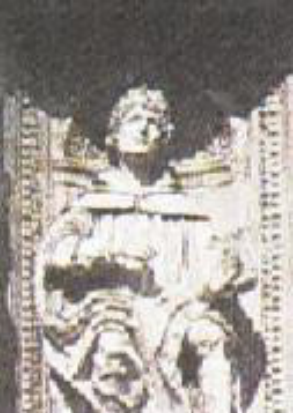
\includegraphics[width=32.55mm,height=113.45mm]{../../images/llm/page_014_img_01.png}%
\end{textblock*}

\end{document}
